\subsection*{\Large Общая характеристика работы}
\fontsize{14pt}{15pt}\selectfont
\subsubsection*{\large{Актуальность темы}}

Взаимодействие различных компонент приложений часто реализуется с помощью встроенных языков: приложение, созданное на одном языке, генерирует код на другом языке и передаёт этот код на выполнение в соответствующее окружение. Примерами могут служить динамические SQL-запросы к базам данных в Java-коде или формирование HTML-страниц в PHP-приложениях. Генерируемый код собирается из строк таким образом, чтобы в момент выполнения результирующая строка представляла собой корректное выражение на соответствующем языке. Такой подход весьма гибок, так как позволяет использовать для формирования выражений различные строковые операции (replace, substring и т.д.) и получать части кода из различных источников (например, учитывать текстовый ввод пользователя, что часто используется для задания фильтров при конструировании SQL-запросов). Кроме того, использование динамически формируемых строковых выражений избавлено от дополнительных накладных расходов, присущих, например, таким технологиям, как ORM, что позволяет достичь высокой производительности. 

Однако динамически формируемые выражения часто конструируются посредством конкатенации в циклах, ветках условных операторов или рекурсивных процедурах, что приводит к получению множества возможных вариантов для каждого выражения в момент выполнения. При этом фрагменты кода на встроенных языках воспринимаются компилятором исходного языка как простые строки, не подлежащие дополнительному анализу. Невозможность статической проверки корректности формируемого выражения приводит к высокой вероятности возникновения ошибок во время выполнения программы. В худшем случае такая ошибка не приведет к прекращению работы приложения, что указало бы на проблемы, однако целостность данных при этом может оказаться нарушена. Более того, использование динамически формируемых выражений затрудняет как разработку информационных систем, так и реижиниринг уже созданных. Для реинжинирига важно иметь возможность изучать систему и модифицировать её, сохраняя функциональность. Однако, например, при наличии в коде приложения встроенного SQL нельзя, не проанализировав все динамически формируемые выражения, точно ответить на вопрос о том, с какими элементами базы данных не взаимодействует система, и  удалить их. При переносе такой системы на другую СУБД необходимо гарантировать, что для всех динамически формируемых выражений значение в момент выполнения будет корректным кодом на языке новой СУБД. С другой стороны, распространённой практикой при написании кода является использование интегрированных сред разработки, производящих подсветку синтаксиса и автодополнение, сигнализирующих о синтаксических ошибках, предоставляющих возможность проводить рефакторинг кода. Такая функциональность значительно упрощают процесс разработки и отладки приложений и полезна не только для основного языка, но и для встроенных языков. Для решения таких задач необходимы инструменты, проводящие статический анализ множества выражений, которые могут быть получены на этапе исполнения из строковых выражений исходного языка.  

Проблема статического анализа динамически формируемых выражений активно исследуется. Большинство работ используют анализ регулярного множества (регулярной аппроксимации), приближающего множество значений динамически формируемого выражения. При этом, как правило, рассматривается вопрос корректности генерируемых выражений или ищутся фрагменты кода, уязвимые для SQL-инъекций. Сильная специализация таких решений не позволяет применять их для других задач. В исследованиях Кюнг-Гу Дох (Kyung-Goo Doh) предлагается комбинация анализа потока данных и синтаксического анализа на основе LR-алгоритма и поднимается вопрос о семантическом анализе встроенных языков. Предлагается использовать классический для LR-анализа механизм атрибутных грамматик, однако, опускается вопрос ресурсоёмкости данного подхода при сложных видах анализа. В работах А. Бреслава рассматривается подход, основанный на построении регулярной аппроксимации множества возможных значений и последующем анализе с использованием обобщённого LR-алгоритма, что кроме расширения класса поддерживаемых языков даёт дополнительные преимущества при переиспользовании структур данных, характерных для обобщённого анализа. Однако, эффективное хранение результатов разбора и оптимизация управления стеком разбора не рассмотрены. Существует также ряд инструментов для работы с динамически формируемыми выражениями: Alvor и IntelliLang, предоставляющие поддержку встроенных языков в интегрированных средах разработки, JSA и PHPSA, позволяющие искать ошибки в выражениях на встроенных языках, SQLWays, поддерживающий трансформацию выражений на встроенных языках, SAFELI --- инструмент статического анализа, предназначенный для определения возможности SQL-инъекций в Web-приложениях и некоторые другие. Однако, эти инструменты либо не поддерживают часто встречающиеся на практике способы формирования выражений, либо имеют существенные ограничения по функциональности: не поддерживают сложные способы формирования строковых выражений, решают только одну узкую задачу (например, проверку корректности, поиск уязвимых конструкций) и т.д. 

\subsubsection*{\large{Цель диссертационной работы}}

Целью данной работы является создание подхода к статическому синтаксическому анализу динамически формируемых выражений, позволяющего обрабатывать произвольную регулярную аппроксимацию без потери точности, а также разработать технологию для создания инструментов статического анализа встроенных текстовых языков, реализующей данный алгоритм.

\subsubsection*{\large{Результаты, выносимые на защиту}}
\begin{enumerate}
    \item Разработан алгоритм синтаксического анализа динамически формируемых выражений, позволяющий обрабатывать произвольную регулярную аппроксимацию множества значений выражения в точке выполнения, реализующий 
    эффективное управление стеком и гарантирующий конечность представления леса вывода. Доказана завершаемость и корректность предложенного алгоритма при анализе регулярной аппроксимации, представимой в виде произвольного конечного автомата без $\varepsilon$-переходов. 
    \item Создана архитектура инструментария для разработки программных средств статического анализа динамически формируемых строковых выражений.
    \item Разработан метод реинжиниринга встроенного программного кода в проектах по реинжинирингу информационных систем. 
\end{enumerate}

\subsubsection*{\large{Методы исследования}}

В работе используется алгоритм обобщённого восходящего синтаксического анализа RNGLR, созданный Элизабет Скотт (Elizabeth Scott) и Адриан Джонстон (Adrian Johnstone) из университета Royal Holloway (Великобритания). Для компактного хранения леса вывода использовалась структура Shared Packed Parse Forest (SPPF), которую предложил Ян Рекерс (Jan Rekers, University of Amsterdam).

    Доказательство завершаемости и корректности предложенного алгоритма проводилось с применением теории формальных языков, теории графов и теории сложности алгоритмов. Приближение множества значений динамически формируемого выражения строилось в виде регулярного множества, описываемого с помощью конечного автомата.

    Апробация созданного подхода проводилась в рамках промышленного проекта компании ЗАО “Ланит-Терком” (Россия) по переносу хранимого кода, содержащего большое количество динамического SQL, с MS SQL Server на Oracle Server. Предложенный в работе алгоритм апробирован в рамках инфраструктуры проекта ReSharper компании ООО “Интеллиджей Лабс” (Россия).

\subsubsection*{\large{Научная новизна}}

На текущий момент существует несколько подходов к анализу динамически формируемых строковых выражений. Некоторые из них, такие как JSA, предназначены только для проверки корректности выражений, основанной на решении задачи о включении одного языка в другой. Выполнение более сложных видов анализа, трансформаций или построения леса разбора не предполагается. В работах А. Бреслава и Кюнг-Гу Дох (Kyung-Goo Doh) рассматривается применение механизмов синтаксического анализа для работы с динамически формируемыми выражениями, однако не решается вопрос эффективного представления результатов разбора. Предложенный в диссертации алгоритм предназначен для синтаксического анализа динамически формируемых выражений и построения компактной структуры данных, содержащей для всех корректных значений выражения их деревья вывода. Это позволяет как проверять корректность анализируемых выражений, так и проводить более сложные виды анализа, используя деревья вывода, хранящиеся в построенной структуре данных.

Большинство существовавших готовых инструментов для анализа динамически формируемых строковых выражений (JSA, PHPSA, Alvor и т.д.), как правило, предназначены для решения конкретных задач в рамках конкретных языков. Решение новых задач или поддержка других языков с помощью этих инструментов затруднено ввиду ограничений, накладываемых архитектурой и возможностями используемого алгоритма анализа. В рамках работы предложена архитектура инструментального средства, включающего предложенный алгоритм и позволяющего упростить создание новых инструментов для анализа динамически формируемых выражений на любых языках программирования (различные диалекты SQL, HTML, JSON и т.д.).

\subsubsection*{\large{Практическая ценность}}

На основе полученных в работе научных результатов был разработан инструментарий (SDK), предназначенный для создания средств статического анализа динамически формируемых выражений. В данный инструментарий входят следующие компоненты: генератор лексических анализаторов, генератор синтаксических анализаторов, библиотеки времени выполнения, реализующие соответствующие алгоритмы анализа, набор интерфейсов и вспомогательных функций для реализации конечного инструмента. Набор генераторов позволяет по описанию лексики и синтаксиса языка строить синтаксический и лексический анализатор, обрабатывающий аппроксимацию множества значений динамически формируемого выражения на соответствующем языке, представленную в виде произвольного конечного автомата. Устранение эпсилон-переходов, необходимое для корректной работы синтаксического анализа, происходит на этапе лексического анализа.

Данный инструментарий позволяет автоматизировать создание лексических и синтаксических анализаторов при разработке программных средств, использующих регулярную аппроксимацию для приближения множества значений динамически формируемых выражений. Инструментарий может использоваться  для решения задач реижинирига --- изучения и инвентаризации систем, поиска ошибок в исходном коде, автоматизации трансформации выражений на встроенных языках. Также данный инструментарий может использоваться при реализации поддержки встроенных языков в интегрированных средах разработки.

Разработанная методика обработки динамического SQL основана на использовании инструментария в качестве генератора для создания лексического и синтаксического анализатора для динамически формируемых выражений по соответствующим спецификациям. В случае динамического SQL могут быть переиспользованы ранее разработанные спецификации. Построение регулярной аппроксимации выделяется в отдельный шаг и производится с помощью анализов, реализованных для обработки основного кода. После завершения синтаксического разбора, анализ леса проводится в основном с помощью тех же методов, что и анализ основного кода, что достигается за счёт идентичности структур деревьев. Данная методика может быть переиспользована для работы с произвольными встроенными текстовыми языками.


\subsubsection*{\large{Апробация работы и публикации}}

С использованием разработанного инструментария было реализовано расширение к инструменту ReSharper (компания ООО ``ИнтеллиДжей Лабс'', Россия), предоставляющее поддержку встроенного T-SQL в проектах на языке программирования C\# в среде разработки Microsoft Visual Studio. Была реализована следующая функциональность: статическая проверка корректности выражений и подсветка ошибок, подсветка синтаксиса и подсветка парных элементов. Исходный код разработанного инструментария и расширения доступен в репозитории по адресу \url{https://github.com/YaccConstructor/YaccConstructor}.

Так же была проведена апробация результатов работы на промышленном проекте по переносу хранимого SQL-кода с MS-SQL Server 2005 на Oraclе 11gR2 (ЗАО ``Ланит-Терком''). Исходная система состояла из 850 хранимых процедур и содержала более 3000 динамических запросов на 2,7 млн. строк хранимого кода. Более половины динамических запросов были сложными и формировались с использованием от 7 до 212 операторов. При этом, среднее количество операторов для формирование запроса ---  40. Реализованный механизм позволил корректно автоматически обработать примерно 45\% запросов и существенно упростил ручную доработку системы. 

Основные результаты работы были доложены на ряде научно-практических конференциях: SECR-2012, SECR-2013, SECR-2014, TMPA-2014, Parsing@SLE-2013, Рабочий семинар ``Наукоемкое программное обеспечение'' при конференции PSI-2014. Доклад на SECR-2014 награждён премией Бертрана Мейера за лучшую исследовательскую работу в области программной инженерии. Разработка инструментальных средств на основе предложенного алгоритма была поддержана Фондом содействия развитию малых форм предприятий в технической сфере (программа УМНИК).
Результаты диссертации изложены в 6 научных работах из которых 3~\cite{1,2,3} опубликованы в журналах из списка ВАК. Работы~\cite{1, 2, 4, 5, 6} написаны в соавторстве. 

В~\cite{1} С. Григорьеву принадлежит реализация ядра платформы YaccConstructor. В~\cite{2} и~\cite{5} Григорьеву С. принадлежит постановка задачи, формулирование требований к разрабатываемым инструментальным средствам. В~\cite{4} автору принадлежит идея, описание и реализация анализа встроенных языков на основе RNGLR алгоритма.  В~\cite{6} Григорьеву С. принадлежит реализация инструментальных средств, проведение замеров, работа над текстом.



\subsubsection*{\large{Объем и структура работы.}} Диссертация состоит из~введения, шести глав, заключения и~списка литературы. Полный объем диссертации \textbf{122}~страницы текста с~\textbf{30}~рисунками и~6~таблицами. 
Список литературы содержит \textbf{66}~наименований.

\newpage
\subsection*{\Large Содержание работы}
Во \underline{\textbf{введении}} обосновывается актуальность исследований, проводимых в рамках данной диссертационной работы, приводится обзор научной литературы по изучаемой проблеме, формулируется цель, 
ставятся задачи работы, сформулированы научная новизна и практическая значимость представляемой работы.


В \underline{\textbf{первой главе}} проводится обзор области исследования. Рассматриваются подходы к анализу динамически формируемых строковых 
выражений и соответствующих инструментов. Кроме того, описывается алгоритм обобщённого восходящего синтаксического анализа RNGLR, положенный в основу алгоритма, предложенного в данной работе. Также описываются 
проекты YaccConstructor и ReSharper SDK, использующиеся в качестве основы разработанного инструментального пакета. 

Во \underline{\textbf{второй главе}} задача синтаксического анализа динамически формируемых выражений формализуется следующим образом: \textit{ для данной однозначной контекстно-свободной грамматики $G = \langle T, N, P, S \rangle$ и детерминированного конечного автомата без $\varepsilon$-переходов $M=(Q,\Sigma,\delta,q_0,q_f)$ такого, что $\Sigma \subseteq T$, необходимо построить конечную структуру данных $F$, содержащую деревья вывода в $G$ всех цепочек $\omega \in L(M)$, корректных относительно грамматики $G$, и не содержащую других деревьев. } Иными словами, необходимо построить алгоритм $\mathbb{P}$ такой, что
    $$(\forall \omega \in L(M)) (\omega \in L(G) \Rightarrow (\exists t \in \mathbb{P}(L(M),G))AST(t, \omega, G))$$
    $$\land (\forall t \in \mathbb{P}(L(M),G))(\exists \omega \in L(M))AST(t,\omega,G).$$ 
    Здесь $AST(t,\omega,G)$ --- это предикат, который истинен, если $t$ является деревом вывода $\omega$ в грамматике $G$.


Так как $\mathbb{P}$ игнорирует ошибки, то будем называть его алгоритмом \textit{ослабленного} (relaxed) синтаксического анализа регулярной аппроксимации динамически формируемого выражения.

Далее описывается алгоритм, её решающий, --- алгоритм синтаксического анализа регулярного множества на основе RNGLR, строящий конечную структуру данных, содержащую деревья вывода для всех цепочек анализируемового множества, 
и формулируется и доказывается ряд вспомогательных определений и утверждений, необходимых для доказательства основных утверждений о корректности предложенного алгоритма.

\textsc{Определение 1.} 
\emph{Корректное дерево}~--- это упорядоченное дерево со следующими свойствами.
\begin{enumerate}
  \item Корень дерева соответствует стартовому нетерминалу грамматики $G$.
  \item Листья соответствуют терминалам грамматики $G$. Упорядоченная последовательность листьев соответствует некоторому пути во входном графе.
  \item Внутренние узлы соответствуют нетерминалам грамматики $G$. Дети внутреннего узла (для нетерминала $N$) соответствуют символам правой части некоторой продукции для $N$ в грамматике $G$.
\end{enumerate}

\textsc{Лемма.}
\textit{Пусть обрабатывается внутренний граф $\mathcal{G}=(V,E)$. Тогда для каждого ребра GSS $(v_{t}, v_{h})$ такого, что $v_{t} \in V_{t}.processed$, $v_{h} \in V_{h}.processed$, где $V_{t} \in V$ и $V_{h} \in V$, терминалы ассоциированного поддерева соответствуют некоторому пути из вершины $V_{h}$ в $V_{t}$ в графе $\mathcal{G}$.}

\vspace{10pt}

Сформулированы и доказаны три теоремы о завершаемости и корректности предложенного алгоритма.

\vspace{5pt}

\textsc{Теорема 1.} 
\textit{Алгоритм завершает работу для любых входных данных.}

\vspace{10pt}

\textsc{Теорема 2.} 
\textit{Любое дерево, извлечённое из SPPF, является корректным.}

\vspace{10pt}

\textsc{Теорема 3.} 
\textit{Для каждой строки, соответствующей пути $p$ во входном графе, и выводимой в эталонной грамматике $G$, из SPPF может быть извлечено корректное дерево $t$. То есть $t$ будет являться деревом вывода цепочки, соответствующей пути $p$, в грамматике $G$.}

\vspace{10pt}

В \underline{\textbf{третьей главе}}  описывается инструментальный пакет YC.SEL.SDK, 
разработанный в ходе данной работы на основе алгоритма, описанного во второй главе. YC.SEL.SDK предназначен для разработки инструментов анализа динамически формируемых выражений. Описывается архитектура 
компонентов и особенности их реализации. Также описывается YC.SEL.SDK.ReSharper --- обёртка над YC.SEL.SDK, позволяющая создавать расширения к ReSharper для поддержки встроенных языков.

В \underline{\textbf{четвёртой главе}} описывается метод реинжиниринга встроенного программного кода.

В \underline{\textbf{пятой главе}} приводятся результаты экспериментального исследования YC.SEL.SDK.

Реализованный инструментарий был апробирован в рамках промышленного проекта по миграции базы данных с MS-SQL Server 2005 на Oraclе 11gR2, что позволило апробировать как предложенную архитектуру, так и протестировать некоторые части инструментария на реальных данных.

Обрабатываемая система состояла из 850 хранимых процедур и содержала около 2,6 миллионов строк кода. В ней присутствовало 2430 точек выполнения динамических запросов, из которых больше 75\% могли принимать 
более одного значения и при их формировании использовалось от 7 до 212 операторов. При этом среднее количество операторов для формирования запроса равнялось 40.

Так как анализатор T-SQL был разработан ранее в рамках проекта, в котором происходило внедрение, то для создания анализатора встроенного SQL была использована готовая грамматика и по ней построен 
синтаксический анализатор. Построение регулярной аппроксимации и лексический анализ также были реализованы ранее в рамках основного проекта и были переиспользованы. 
Далее были реализованы функции вычисления метрик и вывода результата, после чего полученная функциональность была встроена в существующую цепочку обработки основного кода.

Алгоритм успешно завершил работу на 2188 входных графах, аппроксимирующих множества значений запросов. Ручная проверка входных графов, на которых алгоритм завершался с ошибкой, показала, что они действительно не содержали ни одного корректного в эталонном языке выражения. Причиной этого стала либо некорректная работа лексического анализатора, либо наличие в выражениях конструкций, не поддержанных в существующей грамматике. Так как лексический анализатор и грамматика были полностью заимствованы из оригинального проекта, то наличие этих ошибок не является недоработками алгоритма синтаксического анализа. Общее время синтаксического анализа составило 27 минут, из них 13 минут было затрачено на разбор графов, не содержащих ни одного корректного выражения. Из них 256 секунд --- обработка одного графа (5747 рёбер и 3897 вершин), прерванная по таймауту. Дальнейшие значения приводятся только для графов, которые удалось проанализировать. 604 из этих графов прождали ровно одно значение и анализировалось не более 1 миллисекунды. На разбор 1790 графов ушло не более 10 миллисекунд. На анализ двух графов было затрачено более 2 минут: 152,215 и 151,793 секунд соответственно. Первый граф содержал 2454 вершин и 54335 рёбер, второй~--- 2212 вершин и 106020 рёбер. Распределение входных графов по промежуткам времени, затраченных на анализ, приведено на графике на рисунке~\ref{distr}.

\begin{figure}[H]
  \centering
 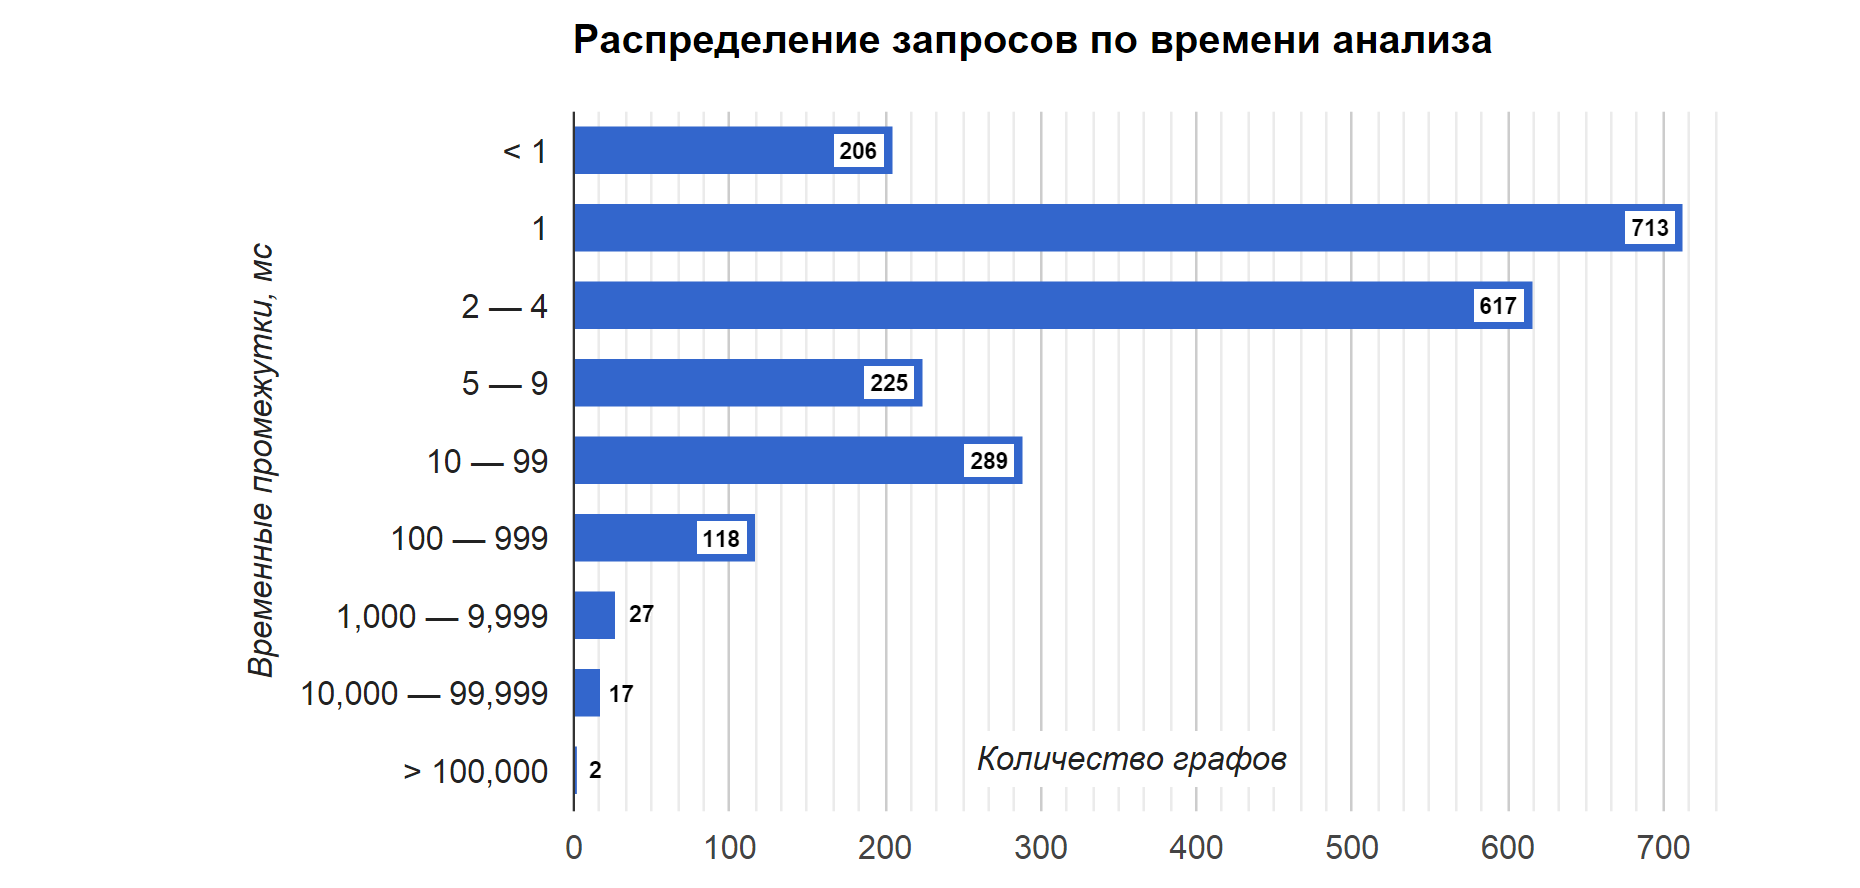
\includegraphics[width=0.95\textwidth]{distr.png}
 \caption{Распределение запросов по времени анализа}
 \label{distr}
\end{figure}



\begin{figure}[h!]
 \centering
 \includegraphics[width=0.95\textwidth]{AlvorVsYC.eps}
 \caption{Сравнение производительности Alvor и синтаксического анализатора на базе YC.SEL.SDK}
 \label{fig:YCvsAlvor}
\end{figure}


\underline{\textbf{Шестая глава}} содержит результаты сравнения и соотнесения реализованного алгоритма с основными существующими аналогами.

В \underline{\textbf{заключении}} приведены основные результаты работы, которые заключаются в следующем.
\begin{enumerate}
    \item Разработан алгоритм синтаксического анализа динамически формируемых выражений, позволяющий обрабатывать произвольную регулярную аппроксимацию множества значений выражения в точке выполнения, реализующий 
    эффективное управление стеком и гарантирующий конечность представления леса вывода. Доказана завершаемость и корректность предложенного алгоритма при анализе регулярной аппроксимации, представимой в виде произвольного конечного автомата без $\varepsilon$-переходов.
    \item Создана архитектура инструментария для разработки программных средств статического анализа динамически формируемых строковых выражений.
    \item Разработан метод реинжиниринга встроенного программного кода в проектах по реинжинирингу информационных систем. Данный метод применён в проекте компании ЗАО ``Ланит-Терком'' по переносу информационной системы с MS-SQL Server на Oracle Server, для чего реализованы соответствующие программные компоненты.
\end{enumerate}

Кроме того, реализован инструментальный пакет для разработки средств статического анализа динамически формируемых выражений. На его основе реализован плагин для ReSharper. Код опубликован на сервисе GitHub: \\ \url{https://github.com/YaccConstructor/YaccConstructor}.

В дальнейшем планируется развитие платформы и плагина. На уровне платформы необходимо реализовать механизмы, требующиеся для трансформаций кода на встроенных языках. Механизмы трансформации встроенных языков требуются для проведения миграции с одной СУБД на другую или для миграции на новые технологии, например, LINQ. Эта задача связана с двумя проблемами: возможностью проведения нетривиальных трансформаций и доказательство корректности трансформаций. Планируется реализация проверки корректности типов. Для SQL это должна быть как проверка типов внутри запроса, так и проверка того, что тип возвращаемого запросом результата соответствует типу хост-переменной, выделенной для сохранения результата в основном коде.

Более общей проблемой, подлежащей дальнейшему исследованию, является возможность выполнения семантических действий непосредственно над SPPF. Это необходимо для рефакторинга, улучшения качества трансляции, автоматизации перехода на более надёжные средства метапрограммирования.

Важной задачей является теоретическая оценка сложности предложенного алгоритма синтаксического анализа. В известных работах не приводится строгих оценок подобных алгоритмов, поэтому данная задача является самостоятельным исследованием.

С целью обобщения предложенного подхода к синтаксическому анализу, а также для получения лучшей производительности и возможностей для более качественной диагностики ошибок, планируется переход на алгоритм обобщённого LL-анализа (GLL). Планируется исследовать возможность улучшения предложенного алгоритма при переходе на другие алгоритмы обобщённого LR-анализа, например, такие как BRNGLR и RIGLR.

Кроме того, важной задачей является реализация диагностики ошибок, решение которогй для обобщённого восходящего анализа активно исследуется. Адоптация предложенных решений для пименеия в пердставленном алгоритме требует отдельной работы.


\newpage
\renewcommand{\refname}{\Large Публикации автора по теме диссертации}
%\nocite{*}
%\bibliography{biblio}

\begin{thebibliography}{99}

\bibitem{1} Кириленко Я. А., Григорьев С. В., Авдюхин Д. А. Разработка синтаксических анализаторов в проектах по автоматизированному реинжинирингу информационных систем. Научно-технические ведомости Санкт-Петербургского государственного политехнического университета информатика, телекоммуникации, управление. Т. 3, N 174, 2013. C. 94 --- 98.
\bibitem{2} Григорьев С. В., Вербицкая Е. А., Полубелова М. И., Иванов А. В., Мавчун Е. В. Инструментальная поддержка встроенных языков в интегрированных средах разработки. Моделирование и анализ информационных систем. Т. 21, N 6, 2014. С. 131---143.
\bibitem{3} Григорьев С. В. Алгоритм синтаксического анализа динамически формируемых выражений.

\bibitem{4}Semen Grigorev, Iakov Kirilenko. GLR-based abstract parsing. In Proceedings of the 9th Central \& Eastern European Software Engineering Conference in Russia (CEE-SECR ’13). 2013. ACM, New York, NY, USA. 1-9 p.
\bibitem{5}Semen Grigorev, Ekaterina Verbitskaia, Andrei Ivanov, Marina Polubelova, Ekaterina Mavchun. String-embedded language support in integrated development environment. In Proceedings of the 10th Central and Eastern European Software Engineering Conference in Russia (CEE-SECR '14). 2014. ACM, New York, NY, USA. 1-11 p.
\bibitem{6}Semen Grigorev, Iakov Kirilenko. From Abstract Parsing to Abstract Translation. Proceedings of the Spring/Summer Young Researchers' Colloquium on Software Engineering. 2014. Saint Petersburg, Russia. 1-5 p.

\end{thebibliography}
